\section{Introduction}\label{sec:intro}
Despite their success deep neural networks (DNNs) are still largely considered as black boxes.  The main issue is that in each layer of a DNN, the linear computation, i.e., multiplication by the weight matrix  and the non-linear activations are entangled. Such entanglement has its \emph{pros} and \emph{cons}. The commonly held view  is that such entanglement is the key to success of DNNs, in that, it allows DNNs to learn sophisticated structures in a layer-by-layer manner. However, in terms of interpretability, such entanglement has an adverse effect: only the final layer is linear and amenable to a feature/weight interpretation, and the hidden layers are non-interpretable due to the non-linearities. 

%Prior works \citep{ntk,arora2019exact,cao2019generalization} showed that training an infinite width DNN with gradient descent is equivalent to a kernel method with the so called \emph{neural tangent kernel} matrix which is based on the gradient information. While as a pure kernel method, the NTK matrix performed better than other pure kernel methods, it was an open question in NTK theory to understand why finite width DNNs still outperformed their corresponding NTK \citep{arora2019exact}. %The open question with the NTK theory was to explain why finite width DNNs are better than infinite width NTK \citep{arora2019exact}. 

Prior works \citep{ntk,arora2019exact,cao2019generalization} showed that training an infinite width DNN with gradient descent is equivalent to a kernel method with the so called \emph{neural tangent kernel} matrix which is based on the gradient information. As a pure kernel method, the NTK matrix performed better than other pure kernel methods. However, the NTK theory has the following two issues when it comes to addressing the `black box'-ness:

$\bullet$ \textbf{Issue I:} It was observed that finite width DNNs outperformed their corresponding infinite width NTK matrix \citep{arora2019exact}. This implies the infinite width NTK matrix does not fully explain finite width DNNs, and it was an open question to address this performance gap \citep{arora2019exact}.

$\bullet$ \textbf{Issue II:} The NTK matrix is based on the gradients and hence offers no further interpretation or insight into the inner workings even in the infinite width case.


%\cite{npk} developed a dual view for DNNs with rectified linear units (ReLUs) to exploit the gating property (i.e., `on/off' states) of the ReLUs.  
A dual view for DNNs with rectified linear units (ReLUs) was recently developed by \cite{npk} who exploited the gating property (i.e., `on/off' states) of the ReLUs. The dual view is essentially \emph{linearity in the path space}, i.e., the output is the summation of path contributions.  While the weights in a path are the same for each input, whether or not a path contributes to the output is entirely dictated by the gates in the path, which are `on/off' based on the input. To understand the role of the gates, a deep gated network (DGN) (see \Cref{fig:lgln}) was used to \emph{disentangle} the \emph{learning in the gates} from the \emph{learning in weights}. In a DGN,  the gates are generated (and learnt) in a `gating network' which is a DNN with ReLUs and are applied as external signals and the weights are learnt in a `weight network' consisting of \emph{gated linear units} (GaLUs) \citep{sss}. Each GaLU multiplies its pre-activation and the external gating signal. Using the DGN, two important insights were provided in relation to issues with the NTK theory:  

(i) It was shown that learning in the gates is most crucial for finite width networks to outperform infinite width NTK; this addresses \textbf{Issue I}.

(ii) In the infinite width regime, when learning the weights with fixed gates, it was shown that the NTK is equal to (but for a scalar) a so called neural path kernel (NPK) which is a kernel solely based on inputs and gates and is dictated by the gating network. In other words, the interpretation of the weight network is that it is equivalent to the NPK, and since NPK is dictated by the gating network, \textbf{Issue II} gets shifted entirely to interpreting the gating network, i.e., to interpreting the gates as opposed to interpreting the gradients.

\begin{figure}[!t]
\centering
\begin{minipage}{0.9\columnwidth}
\centering
\begin{minipage}{0.49\columnwidth}
\centering

\resizebox{0.8\columnwidth}{!}{
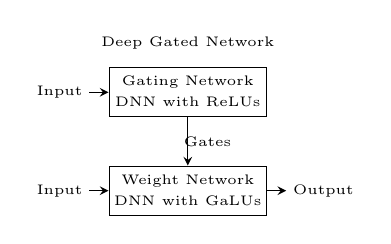
\begin{tikzpicture}

\node []  (fntext)at (5,1) {\tiny{Deep Gated Network}};
%Feature Network
\node [draw,
	minimum width=2cm,
	minimum height=0.625cm,
]  (fnbox)at (5,0.375) {};
\node []  (fntext)at (5,0.5) {\tiny{Gating Network}};

\node []  (fntext)at (5,0.25) {\tiny{DNN with ReLUs}};


%Feature Network Input
\node (fin) [left of=fnbox,node distance=1.25cm, coordinate] {};
\node[left=-1pt] at (fin.west){\tiny{Input}};
\draw[-stealth] (fin.center) -- (fnbox.west);




%Value Network

\node [draw,
	minimum width=2cm,
	minimum height=0.625cm,
]  (vnbox)at (5,-0.875) {};
\node []  (fntext)at (5,-0.75) {\tiny{Weight Network}};
\node []  (vntext)at (5,-1) {\tiny{DNN with GaLUs}};

%Value Network Input
\node (vin) [left of=vnbox,node distance=1.25cm, coordinate] {};
\node[left=-1pt] at (vin.west){\tiny{Input}};
\draw[-stealth] (vin.center) -- (vnbox.west);

%Feature Network Output
\node (vout) [right of=vnbox,node distance=1.25cm, coordinate] {};
\node[right=-1pt] at (vout.west){\tiny{Output}};
\draw[-stealth]  (vnbox.east)--(vout.center);



\draw[-stealth]  (fnbox.south)--(vnbox.north);

\node []  (gates)at (5.25,-0.25) {\tiny{Gates}};


\end{tikzpicture}


}
\end{minipage}
\begin{minipage}{0.49\columnwidth}
\centering

\resizebox{0.8\columnwidth}{!}{
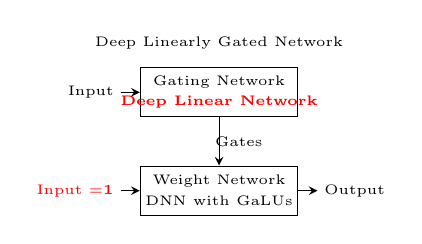
\begin{tikzpicture}

\node []  (fntext)at (5,1) {\tiny{Deep Linearly Gated Network}};
%Feature Network
\node [draw,
	minimum width=2cm,
	minimum height=0.625cm,
]  (fnbox)at (5,0.375) {};
\node []  (fntext)at (5,0.5) {\tiny{Gating Network}};

\node []  (fntext)at (5,0.25) {\tiny{\bf\color{red}{Deep Linear Network}}};


%Feature Network Input
\node (fin) [left of=fnbox,node distance=1.25cm, coordinate] {};
\node[left=-1pt] at (fin.west){\tiny{Input}};
\draw[-stealth] (fin.center) -- (fnbox.west);




%Value Network

\node [draw,
	minimum width=2cm,
	minimum height=0.625cm,
]  (vnbox)at (5,-0.875) {};
\node []  (fntext)at (5,-0.75) {\tiny{Weight Network}};
\node []  (vntext)at (5,-1) {\tiny{DNN with GaLUs}};

%Value Network Input
\node (vin) [left of=vnbox,node distance=1.25cm, coordinate] {};
\node[left=-1pt] at (vin.west){\tiny{\color{red}{Input =$\mathbf{1}$}}};
\draw[-stealth] (vin.center) -- (vnbox.west);

%Feature Network Output
\node (vout) [right of=vnbox,node distance=1.25cm, coordinate] {};
\node[right=-1pt] at (vout.west){\tiny{Output}};
\draw[-stealth]  (vnbox.east)--(vout.center);



\draw[-stealth]  (fnbox.south)--(vnbox.north);

\node []  (gates)at (5.25,-0.25) {\tiny{Gates}};


\end{tikzpicture}


}
\end{minipage}
\end{minipage}
\caption{\small{DGN is a setup to understand the role of gating in DNNs with ReLUs. The DLGN setup completely disentangles and re-arranges the computations in an interpretable manner. The surprising fact that a constant $\mathbf{1}$ input is given to weight network of DLGN is justified by theory and experiments in \Cref{sec:analysis,sec:dlgn}.}}
\label{fig:lgln}
\end{figure}

\textbf{Contribution I.}  In this paper, we extend the dual view with a focus on `black box'-ness. Our contributions are listed below.

$\bullet$\textbf{Extending Dual View}(\Cref{sec:analysis}).  We present an unnoticed insight in prior work on fully connected networks that the \textbf{NPK is a product kernel} and is invariant to layer permutations. We extend the dual view to show that the NPK is rotationally invariant in the presence of convolutions with global average pooling, and NPK is an ensemble of many kernels in the presence of skip connections. 

$\bullet$ \textbf{Disentangling Using Dual View}(\Cref{sec:dlgn}). To address  `black box'-ness, we disentangle the `gating network' as well as `weight network'. For this, we propose a novel Deep \emph{Linearly} Gated Network (DLGN) as a \emph{mathematically interpretable} counterpart of a DNN with ReLUs (see \Cref{fig:lgln}).  In a DLGN, the gating network is a deep linear network, i.e., there are no non-linear activations. Thus, the transformation from input to the pre-activations are linear matrix operations; this \emph{disentangles the gating network}. We then argue via theory and experiments that the  \emph{weight network is disentangled in the path space}. For this, we experimentally show that, destroying the layer-by-layer structure by permuting the layers and providing a constant $\mathbf{1}$ as input (see DLGN in \Cref{fig:lgln}) do not  degrade performance. These counter intuitive and surprising results are difficult to reconcile using the commonly held `sophisticated structures are learnt in layers' interpretation. However, these experimental results follow from theoretical results and insights in \Cref{sec:analysis}.  In other words, the right approach is to think that learning in the weight network happens path-by-path, which is interpreted via the NPK. Using the fact that NPK is solely based on input and the gates, and the fact that, in a DLGN, the pre-activation to the gates are linearly functions of the input, we have complete disentanglement.% and interpretability.

\textbf{Message.} The DLGN is not an alternative architecture per se, but a disentanglement and an interpretable re-arrangement of the computations in a DNN with ReLUs. The DLGN disentangles the computations into two  `mathematically' interpretable linearities (i) the `primal' linearity between the input and the pre-activations in the gating network and (ii) the `dual' linearity in the path space in the weights network. Dual linearity is characterised by the NPK which is based on input and gates. We compare the performance of DNN, DGN and DLGN on CIFAR-10 and CIFAR-100 to show that, the DLGN recovers more than $83.5\%$ of the performance of the DNN, i.e., while entanglement in the DNNs enable their improved performance,  the `disentangled and interpretable'  computations in the DLGN can still recover most part of the performance. This brings us to an interesting question: `Is a DLGN a universal spectral approximator?' (see \Cref{sec:dlgn}).

%\textbf{Contribution II.} We show the usefulness of the dual view by answering the following open question in \citep{randlabel}: \emph{when trained upstream with random labels followed by downstream training with true labels, the test accuracy degrades, why?} We show that the degradation is because the gates. We show the usefulness of the dual view by answering the following open question in \citep{randlabel}: \emph{when trained upstream with random labels followed by downstream training with true labels, the test accuracy degrades, why?} We show that the degradation is because the gates. We show the usefulness of the dual view by answering the following open question in \citep{randlabel}: \emph{when trained upstream with random labels followed by downstream training with true labels, the test accuracy degrades, why?} We show that the degradation is because the gates.

% and not the weights. %We also show that in the \emph{external-fixed gates} setting, using the gates from a pre-trained DNN and then training the weights first upstream with random labels 
\textbf{Related Works.} We now compare our work with the related works.\\
$\bullet$ \textbf{Kernels.} Several works have examined theoretically as well as empirically two important kernels associated with a DNN namely its NTK based on the correlation of the gradients and the conjugate kernel based on the correlation of the outputs \citep{spectra,laplace,belkin,genntk,disentangling,ntk,arora2019exact,convgp,fcgp,lee2020finite}. In contrast, the NPK is based on the correlation of the gates. We do not build pure-kernel method with NPK, but use it as an aid to disentangle finite width DNN with ReLUs.\\  %It was shown in [\citenum{li2019enhanced}], that  prediction using CNTK with GAP is equivalent to prediction using CNTK without GAP but with full translation data augmentation with wrap-around at the boundary. This is related to \Cref{th:mainconv}. It was shown in [\citenum{veit2016residual}] that residual networks behave like ensemble of shallow networks. This is related \Cref{th:mainres}.
%\textbf{Random Labels.} In [\citenum{randlabel}], both positive and negative effects on downstream training performance due to upstream training with random labels was studied. The question of why the test performance degrades due to upstream training with random labels was left open, which we addressed in our paper. 
$\bullet$ \textbf{ReLU, Gating, Dual Linearity.} A spline theory based on max-affine linearity was proposed in \citep{balestriero2018spline,balestriero2018hard} to show that a DNN with ReLUs performs hierarchical, greedy template matching. In contrast, the dual view exploits the gating property to simplify the NTK into the NPK. Gated linearity was studied in \citep{sss} for single layered networks, along with a non-gradient algorithm to tune the gates. In contrast, we look at networks of any depth, and the gates are tuned via standard optimisers. The main novelty in our work in contrast to the above is that in DLGN the feature generation is linear. The gating in this paper refers to the gating property of the ReLU itself and has no connection to \citep{highway}  where gating is a mechanism to regulate information flow. Also, the soft-gating used in our work and in \citep{npk} enables gradient flow via the gating network and is different from \emph{Swish} \citep{swish}, which is the multiplication of pre-activation and sigmoid.\\
$\bullet$ \textbf{Finite vs Infinite Width.} \cite{finitevsinfinite} perform an extensive comparison of finite versus infinite width DNNs. An aspect that is absent in their work, but present in the dual view is the disentanglement of gates and weights, and the fact that the learning in gates is crucial for finite width network to outperform infinite width DNNs. In our paper, we make use of theory developed for infinite width DNNs to provide empirical insights into inner workings of finite width networks.\\
$\bullet$ \textbf{Capacity.} Our experiments on destruction of layers, and providing constant $\mathbf{1}$ input are direct consequences of the insights from dual view theory. These are not explained by mere capacity based studies showing  DNNs are powerful to fit even random labelling of datasets \citep{ben}.

\begin{comment}
Learning in gates is also takes away the importance of looking at NPK at randomised initialisation, a reason why we did not pursue the question of analysing the spectrum of NPK at randomised initialisation in the limit of infinite width/depth (like \cite{disentangling,spectra}) or design a pure kernel method (like \cite{arora2019,fcgp,convgp}) or its constancy as in \cite{belkin}. The NTK and NPFs are related at an algebraic level (see \Cref{prop:ntknew}), i.e., the relation holds for any width, depth, and initialisation, and not just in limiting case. Also, our result that convolutions with pooling make the NPFs rotationally invariant is again algebraic and holds for finite width/depth as opposed to an asymptotic analytical characterisation of pooling \cite{disentangle}. Similarly, the sum of product structure of ResNets is also an algebraic result as opposed to \cite{meanres} which shows that ResNets are an ensemble of shallow architecture by ignoring certain higher order terms in the mean-field analysis. \cite{loss} study the dynamics of NTK empirically and show that its performance matches that of full network training in $15\%$ to $45\%$ of training time. The fact that NPF/NPK/gates learning is continuous ($\text{NTK}^{\text{gate-learn}}$ dictates the dynamics of the gates) and that learnt NPF/NPK/gates perform as well as the original DNN was already empirically shown by \cite{npk}, and our experiments add strength for the same. 

Several recent works \cite{disentangling,nth,meanres,deepres,spectra,laplace,belkin,loss} have looked at the NTK. We are primarily interested in a pedagogical nugget that helps us to interpret DNNs with ReLU. Our work is based on duality \cite{npk} which differs at a conceptual level from the aforementioned works in the following ways: (i) firstly the role of ReLU is explicitly accounted by encoding them as NPFs, (ii) the connection between the NTK and NPF is algebraic (see \Cref{prop:ntknew}) and not just in the limiting case (iii) as per theory (\Cref{th:main}) so long as the weights of the value network are random and statistically decoupled from NPFs, the NPV do not play an important role and a fact which is also verified experimentally where using the NPFs alone the NPV could be trained from scratch (iv) the NPK can correspond to arbitrary finite width feature network weights (see remark on role of activations in \Cref{sec:fc}) and not just random.  Our experiments (as well as those by \cite{npk}) showing that learning in the gates is the difference between NTK and finite width DNNs is the key differentiator from \cite{nth,label} which also looked at difference between finite width DNNs and NTK. The learning in gates is also takes away the importance of looking at NPK at randomised initialisation, a reason why we did not pursue the question of analysing the spectrum of NPK at randomised initialisation in the limit of infinite width/depth (like \cite{disentangling,spectra}) or design a pure kernel method (like \cite{arora2019,fcgp,convgp}) or its constancy as in \cite{belkin}. Further, we believe that the NPK at randomised initialisation might also be associated with a simpler kernel in manner to the result that (\cite{laplace}) NTK for FC-DNN with ReLU  is closely related to the standard Laplace kernel. Our result that convolutions with pooling make the NPFs rotationally invariant is again algebraic and holds for finite width/depth as opposed to an asymptotic analytical characterisation of pooling \cite{disentangle}. Similarly, the sum of product structure of ResNets is also an algebraic result as opposed to \cite{meanres} which shows that ResNets are an ensemble of shallow architecture by ignoring certain higher order terms in the mean-field analysis. \cite{loss} study the dynamics of NTK empirically and show that its performance matches that of full network training in $15\%$ to $45\%$ of training time. The fact that NPF/NPK/gates learning is continuous ($\text{NTK}^{\text{gate-learn}}$ dictates the dynamics of the gates) and that learnt NPF/NPK/gates perform as well as the original DNN was already empirically shown by \cite{npk}, and our experiments add strength for the same. 


\cite{disentangling} (via a spectral analysis of the NTK) show presence of (i) ordered phase, in which the trainability of DNNs degrades at large depths, but their ability to generalise does not and (ii) chaotic phase, in which, trainability improves with depth, but generalisation degrades,  (iii)  pooling  improves the depth over which networks can generalise in the chaotic phase but reduces the depth in the ordered phase. \cite{spectra} show that the eigenvalue distributions of the Conjugate Kernel and Neural Tangent Kernel converge to deterministic limits. In order to explain the difference between the NTK and finite width DNNs, \cite{nth} derive an infinite hierarchy of differential equations known as the neural tangent hierarchy (NTH).  \cite{label} observe that the performance gap between NTK and finite width DNN may be be partly due to the label agnostic nature of the NTK and introduce a novel approach from the perspective of label-awareness to reduce this gap. \cite{meanres} use mean-field analyses of two-layer DNNs to propose several novel training schemes for ResNets that performs well on the standard datasets. \cite{deepres} compare the kernel of deep ResNets with that of deep FFNets and show that the class of functions induced by the kernel of i) FFNets degenerates asymptotically with depth and i) ResNets does not degenerate with depth. \cite{loss} study the dynamics of NTK and show that there is a highly chaotic rapid initial transient phase in which NTK changes rapidly, followed by a phase where the NTK changes at constant velocity, and its performance matches that of full network training in $15\%$ to $45\%$ of training time. \cite{genntk} provide a generalised NTK analysis and show that noisy gradient descent with weight decay can still exhibit a “kernel-like” behaviour. \cite{belkin} show that constancy of the NTK results from the scaling properties of the norm of the Hessian matrix of the network as a function of the network width. \

\textbf{Related to NTK:} \cite{disentangling} (via a spectral analysis of the NTK) show presence of (i) ordered phase, in which the trainability of DNNs degrades at large depths, but their ability to generalise does not and (ii) chaotic phase, in which, trainability improves with depth, but generalisation degrades,  (iii)  pooling  improves the depth over which networks can generalise in the chaotic phase but reduces the depth in the ordered phase. 
\cite{scaling}  propose a theory for infinite width DNNs that connects  mean-field (MF) and constant kernel (NTK) limits. \cite{ntkregression} analyse the high-dimensional asymptotic generalisation performance of kernel regression with the NTK of a single hidden-layer neural network.



 \textbf{Gates and Sub Networks:} \cite{srivastava2014understanding} analysed the role of gates empirically and via a t-SNE based analysis showed that ``subnetworks active for examples of the same class are much more similar to each other compared to the ones activated for the examples of different classes''. They also observe gates flip which is upto $20\%$ of examples in the initial phases of training but quickly settle down to $5\%$. \cite{subnet1}, study active sub-networks at sample level and class level to propose two adversarial example detection methods.

\textbf{Our Work:} In contrast to aforementioned works on NTK, the focus of this paper has been on the NPK which is based on the gates, and instead of a pure kernel method, we use the intuition obtained on the NPK to test a finite width DGN. Further, we believe that the dual view based interpretation is more direct (such as rotational invariance of NPK due to convolutions and pooling, a fact not noticed in prior work). Our empirical results are closely tied to the theory we develop which is absent in prior empirical works that analysed the role of gates and sub-networks.
\end{comment}



%In this paper, we focus on DNNs with rectified linear units (ReLUs), and specifically the gating property (i.e., `on/off') of ReLUs. For such DNNs, we address the issues of entanglement and `black box'-ness by building on the work of \cite{npk} who showed the importance of gating, and also provided a dual view to analytically encode the gates.

%To address the `black box'-ness issues recent works \citep{ntk,arora2019exact,cao2019generalization} have provided a kernel interpretation of DNNs  in terms of the so called \emph{neural tangent kernel} (NTK) matrix which is based on gradient information. As the width increases to infinity, the NTK matrix of a randomly initialised DNN converges to fixed matrix, and training such a DNN with gradient descent is equivalent to a kernel method with this fixed NTK matrix. While the infinite width NTK performed better than other pure kernel methods, finite width DNNs still outperformed their corresponding infinite width NTK \citep{arora2019exact}. The open question with the NTK theory was to explain why finite width DNNs are better than infinite width NTK \citep{arora2019exact}.



%\cite{npk} focussed their attention on DNNs with rectified linear units (ReLUs), and in particular the gates (i.e., `on/off' states) of the ReLUs. They showed that the most crucial learning in a DNN is the learning in the gates by separating the same from the learning in the weights.  For the purpose of analytical characterisation, they developed a dual view in which computations are broken path-by-path.  The input and the gates are encoded in the  \emph{neural path feature} vector and the weights are encoded in the  \emph{neural path value} vector, and the output is the inner product of these two vectors. 

%\cite{npk} focussed their attention on DNNs with rectified linear units (ReLUs), and in particular the gates (i.e., `on/off' states) of the ReLUs. They showed that the most crucial learning in a DNN is the learning in the gates by separating the same from the learning in the weights.  For the purpose of analytical characterisation, they developed a dual view in which computations are broken path-by-path.  The input and the gates are encoded in the  \emph{neural path feature} vector and the weights are encoded in the  \emph{neural path value} vector, and the output is the inner product of these two vectors. They considered an \emph{external-fixed gates} setting to analyse the learning of the weights given the gates:   the gates are generated by a DNN with ReLUs and are applied as external signals and the weights are trained in a network consisting of \emph{gated linear units} (GaLUs) \citep{sss}. Each GaLU multiplies its pre-activation and the external gating signal. Here, they showed that NTK is equal to (but for a scalar) the neural path kernel (NPK) which is the Gram matrix of the neural path features. They also showed that gates (encoded as neural path features) are learnt and such learning in the gates is the reason why finite width networks outperform infinite width NTK, thereby addressing the open question in the NTK theory. It was also shown that the external gates and the weights can be learnt separately and simultaneously to match the performance of DNNs.

%A path starts from an input node, passes through a weight and a gate in each layer and ends at an output node.
%They showed that most crucial learning is to learn to turn the gates `on' or `off' in an input dependent manner. 
%They considered an \emph{external-fixed gates setting} in which they showed that using learnt gates from a pre-trained DNN as external masks and then learning the weights separately in a different network matches the performance of the pre-trained DNN itself.  They also considered a \emph{external-learnable gates setting}, wherein, gates and the weights learnt separately in two different networks performs was only \emph{marginally poor} compared to DNN. 

%To analytically encode the gates, the dual view breaks the computations path-by-path.  A path starts from an input node, passes through a weight and a gate in each layer and ends at an output node. The input and the gates are encoded in the  \emph{neural path feature} vector and the weights are encoded in the  \emph{neural path value} vector, and the output is the inner product of these two vectors. The gates and the neural path features are related: if all the gates in a path are `off', then the neural path feature coordinate corresponding to that path is $0$.  Analytically, the \emph{external-fixed gates setting} is same as fixing the neural path features and learning the neural path value which is characterised by the \emph{neural path kernel} (NPK) which is the Gram matrix of the neural path features.

%The gating plays a central role in DNNs with ReLUs. For a given input, only a subset of gates are `on/active', and the output is produced by the subnetwork made of such active gates and the weights connective them. 


%The NPK is equal to the \emph{Hadamard} product of the input Gram matrix and a correlation matrix which measure the overlap of subnetworks active for various input pairs.


%The dual view breaks down the computations path-by-path. Consider as simple toy network (\Cref{fig:paths}) with an input node, $2$ layer and $2$ hidden units in each layer and an output node. Let the input be $x\in\R$ and the output be $\hat{y}$. This network has $4$ gates (i.e., ReLUs) and $4$ paths. Let us say for this particular input $x$, the bottom ReLU/gate in the first layer is `off/inactive' and rest of the ReLUs are `on/active'. A path is active iff all the gates in the path are active. In this case , paths $p_1$ and $p_2$ are active and paths $p_3$ and $p_4$ are inactive.  The product of the weights in each path is encoded in the so called neural path value $v=(0.1 \cdot 0.2 \cdot 0.7,0.1 \cdot 0.3 \cdot 0.6,-0.1 \cdot 0.4 \cdot 0.7,-0.1 \cdot 0.5 \cdot 0.6)$.  The information in the input and the gates is encoded in the so called neural path feature $\phi(x)= (x\cdot 1, x\cdot 1, x\cdot 0, x\cdot 0)= (x,x,0,0)$, i.e., the coordinates of `on' paths $p_1$ and $p_2$ the signal $x$ at the input node and the coordinates of `off' paths $p_3$ and $p_4$ are $0$. The output is then the inner product of the neural path feature and neural path value, i.e., $\hat{y}(x)=\ip{\phi(x),v}$; this is called \textbf{dual linearity}.

% and expresses the output as the inner product of a `path feature' and a `path value' (both vectors in $\R^{\text{total\,paths}}$).
%A path starts from an input node, passes through a weight and a ReLU in each layer and ends at an output node. 
%A path is `active'  if all the gates in the path are `active' (i.e. `on'). Each path, if active, transmits the signal at its input node, which on its way to the output is scaled by a `path value' which is equal the product of the weights in the path. The `path feature' is the product of signal at the input node and the path activity. 

\begin{comment}
\begin{figure}
\resizebox{.95\columnwidth}{!}{
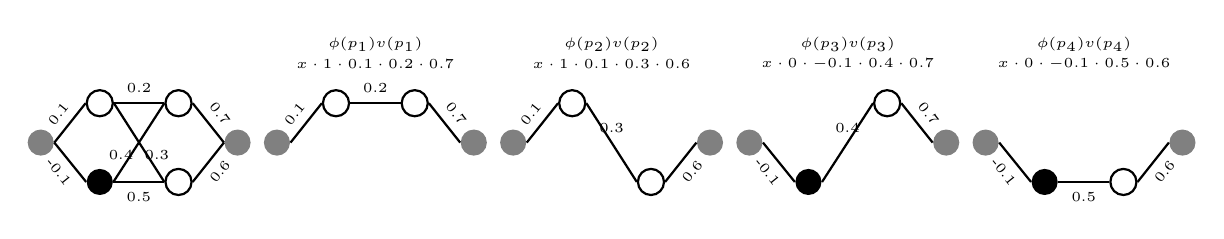
\begin{tikzpicture}
%Top Left
\node[draw,fill=white,circle,thick,
] (tl) at (-0.5,2){};

%Top Right
\node[draw,fill=white,circle,thick,
] (tr) at (0.5,2){};

%Bottom Left
\node[fill=black,circle,
] (bl) at (-0.5,1){};

%Bottom Right
\node[draw,fill=white,circle,thick,
] (br) at (0.5,1){};


%Input
\node[fill=gray,circle,
] (input) at (-1.25,1.5){};


%Output
\node[fill=gray,circle,
] (output) at (1.25,1.5){};

\draw[-, thick] (input.east) -- (tl.west) node [midway, above, sloped] (t1) {\tiny{0.1}};
\draw[-, thick] (input.east) -- (bl.west) node [midway, below, sloped] (t2) {\tiny{-0.1}};
\draw[-, thick] (tl.east) -- (tr.west) node [midway, above, sloped] (t1) {\tiny{0.2}};
\draw[-, thick] (bl.east) -- (br.west) node [midway, below, sloped] (t1) {\tiny{0.5}};
\draw[-, thick] (tl.east) -- (br.west) node [pos=0.85, above] (t1) {\tiny{0.3}};
\draw[-, thick] (bl.east) -- (tr.west) node [pos=0.15, above] (t1) {\tiny{0.4}};
\draw[-, thick] (tr.east) -- (output.west) node [midway, above, sloped] (t1) {\tiny{0.7}};
\draw[-, thick] (br.east) -- (output.west) node [midway, below, sloped] (t1) {\tiny{0.6}};




%%%%%%%%%%%%%%%%%Path 1%%%%%%%%%%%%%%
%Input
\node[fill=gray,circle,
] (p1input) at (1.75,1.5){};


%Output
\node[fill=gray,circle,
] (p1output) at (4.25,1.5){};



%Top Left
\node[draw,fill=white,circle,thick,
] (p1tl) at (2.5,2){};

%Top Right
\node[draw,fill=white,circle,thick,
] (p1tr) at (3.5,2){};




\draw[-, thick] (p1input.east) -- (p1tl.west) node [midway, above, sloped] (t1) {\tiny{0.1}};
\draw[-, thick] (p1tl.east) -- (p1tr.west) node [midway, above, sloped] (t1) {\tiny{0.2}};
\draw[-, thick] (p1tr.east) -- (p1output.west) node [midway, above, sloped] (t1) {\tiny{0.7}};



%%%%%%%%%%%%%%%%%Path 2%%%%%%%%%%%%%%

%Input
\node[fill=gray,circle,
] (p2input) at (4.75,1.5){};


%Output
\node[fill=gray,circle,
] (p2output) at (7.25,1.5){};

%Top Left
\node[draw,fill=white,circle,thick,
] (p2tl) at (5.5,2){};

%Bottom Right
\node[draw,fill=white,circle,thick,
] (p2br) at (6.5,1){};

\draw[-, thick] (p2input.east) -- (p2tl.west) node [midway, above, sloped] (t1) {\tiny{0.1}};
\draw[-, thick] (p2tl.east) -- (p2br.west) node [pos=0.5, above] (t1) {\tiny{0.3}};
\draw[-, thick] (p2br.east) -- (p2output.west) node [midway, below, sloped] (t1) {\tiny{0.6}};



%%%%%%%%%%%%%%%%%Path 3%%%%%%%%%%%%%%

%Input
\node[fill=gray,circle,
] (p3input) at (7.75,1.5){};


%Output
\node[fill=gray,circle,
] (p3output) at (10.25,1.5){};


%Top Right
\node[draw,fill=white,circle,thick,
] (p3tr) at (9.5,2){};

%Bottom Left
\node[fill=black,circle,
] (p3bl) at (8.5,1){};



\draw[-, thick] (p3input.east) -- (p3bl.west) node [midway, below, sloped] (t2) {\tiny{-0.1}};
\draw[-, thick] (p3bl.east) -- (p3tr.west) node [pos=0.5, above] (t1) {\tiny{0.4}};
\draw[-, thick] (p3tr.east) -- (p3output.west) node [midway, above, sloped] (t1) {\tiny{0.7}};


%%%%%%%%%%%%%%%%%Path 4%%%%%%%%%%%%%%

%Input
\node[fill=gray,circle,
] (p4input) at (10.75,1.5){};


%Output
\node[fill=gray,circle,
] (p4output) at (13.25,1.5){};

%Bottom Left
\node[fill=black,circle,
] (p4bl) at (11.5,1){};

%Bottom Right
\node[draw,fill=white,circle,thick,
] (p4br) at (12.5,1){};

\draw[-, thick] (p4input.east) -- (p4bl.west) node [midway, below, sloped] (t2) {\tiny{-0.1}};
\draw[-, thick] (p4bl.east) -- (p4br.west) node [midway, below, sloped] (t1) {\tiny{0.5}};
\draw[-, thick] (p4br.east) -- (p4output.west) node [midway, below, sloped] (t1) {\tiny{0.6}};
%%%%%%%%%%%%%%%%%%%%%%%%%%%%%%

\node[] () at (3,2.75){\tiny{$\phi(p_1)v(p_1)$}};
\node[] () at (3,2.5){\tiny{$x\cdot 1\cdot 0.1 \cdot 0.2 \cdot 0.7$}};

\node[] () at (6,2.75){\tiny{$\phi(p_2)v(p_2)$}};
\node[] () at (6,2.5){\tiny{$x\cdot 1\cdot 0.1 \cdot 0.3 \cdot 0.6$}};

\node[] () at (9,2.75){\tiny{$\phi(p_3)v(p_3)$}};
\node[] () at (9,2.5){\tiny{$x\cdot 0\cdot -0.1 \cdot 0.4 \cdot 0.7$}};

\node[] () at (12,2.75){\tiny{$\phi(p_4)v(p_4)$}};
\node[] () at (12,2.5){\tiny{$x\cdot 0\cdot -0.1 \cdot 0.5 \cdot 0.6$}};




\end{tikzpicture}


}
\caption{Illustration of the dual `path-by-path' view of computations.}
\label{fig:paths}
\end{figure}
\end{comment}

%{\centering \emph{\textbf{How critical is the entanglement for the success of DNNs? or Can we disentangle? }}\par}

%Note that we are not suggesting that we do away with the non-linearity altogether; we are just asking for the disentanglement. In this paper, we focus on DNNs with rectified linear units (ReLUs). For such DNNs, using the dual view of \cite{npk}, we propose a novel way to disentangle the computations into two linear structures. The `black box'-ness issue is resolved because the two linear structures have simple `mathematical' interpretations.  We also show that entanglement is not critical, i.e., our new proposal achieves results comparable to the state of the art.% on standard dataset and at the same time improves interpretability. 

%In this paper, we focus on DNNs with rectified linear units (ReLUs). For such networks, we argue that the `black box'-ness issue is mostly conceptual one arising from the primal view which is partial and incomplete. The primal view is that, increasingly sophisticated features are learnt in a layer-by-layer manner. The conceptual issue here is that, only the final layer is linear and amenable to a feature/weight interpretation, and yet the hidden features i.e., the penultimate layer outputs are not interpretable themselves. 
%The conceptual issue with the primal view is that, only the final layer is linear and amenable to a feature/weight interpretation, and even then, the hidden features i.e., the penultimate layer outputs, obtained as a result of several non-linear operations on the input are not interpretable themselves. 
%Recently \cite{npk} used the \emph{dual view} to investigate the role of gates (i.e., \emph{on/off} state) of the ReLUs. In this paper, we combine the primal dual views to reduce `black box'-ness issue to that of understanding a two linear structure (one each for primal and dual) and a gating mechanism that is sandwidched between the two.

%The dual view proposes an alternative feature decomposition, by projecting the computation onto the dimnesion of the paths. A path starts from an input node, passes through a weight and a ReLU in each layer and ends at an output node. A path is `active' (i.e., `on') if all the gates in the path are `active' (i.e. `on). Each path, if active, transmits the signal at its input node, which on its way to the output is scaled by a `neural path value' (NPV) which is equal the product of the weights in the path. For a given input, a `neural path feature' (NPF) is defined to be the product of signal at the input node and the path activity. The NPF and NPV are vectors in $\R^{\text{total.no.paths}}$, and the ouput is the inner product of these NPF and NPV. Note that the gates dictate the path activity -- the NPFs are known if the input and the gates are known. So, there is no need for any extra procedure to compute the NPFs. 

%The dual view breaks down the computations path-by-path, and expresses the output as the inner product of a `path feature' and a `path value' (both vectors in $\R^{\text{total\,paths}}$).
%The dual view proposes an alternative feature decomposition, by projecting the computation onto the dimnesion of the paths. 
%A path starts from an input node, passes through a weight and a ReLU in each layer and ends at an output node. 
%A path is `active'  if all the gates in the path are `active' (i.e. `on'). Each path, if active, transmits the signal at its input node, which on its way to the output is scaled by a `path value' which is equal the product of the weights in the path. The `path feature' is the product of signal at the input node and the path activity. %The `path feature' and `path value' are vectors in , and the ouput is the inner product of these two. Note that the gates dictate the path activity -- the `path features' are known if the input and the gates are known. So, there is no need for any extra procedure to compute the `path features'. 


%Before we can talk about the practical use of the NPFs, we need to ask "how good are NPFs as features?", i.e., suppose we have the NPFs in hand, is it possible to learn the NPV and if so how effective will be that model. A trivial answer it that in a DNN with ReLUs the NPF and NPV are learnt simultaenous, so NPFs are indeed good features. However, it is also possible to check in a standalone manner as to whether NPFs are good features. This is achieved by a deep gated network (DGN) setup \citep{npk}, where the gates (i.e., NPFs) are generated by in the feature network, and are used as external masks in a different network called the value network (whose weights specify the NPV) which is responsible for the input to the output computation. It was shown that using the gates (i.e., NPFs) from a pre-trained DNN (by letting it to be the feature network), and training the NPV separately in the value network, one can match the performance of the pre-trained DNN. In short, NPFs are indeed useful features.


%Before we can talk about the practical use of the `path features', we need to ask "how good are these as features?", i.e., suppose we have them in hand, is it possible to learn the `path value' and if so how effective will be that model. A trivial answer it that in a DNN with ReLUs the `path feature' and `path value' are learnt in the same network, so `path features' are indeed good. However, it is also possible to check in a standalone manner the goodness of `path features'. This is achieved by a deep gated network (\texttt{DGN}) setup \citep{npk}, where the gates (i.e., `path features') are generated by in the feature network, and are used as external masks in a different network called the value network (whose weights specify the `path value') which is responsible for the input to the output computation. It was shown that using the gates (i.e., `path features') from a pre-trained DNN (by letting it to be the feature network), and training the `path value' separately in the value network, one can match the performance of the pre-trained DNN. In short, `path features' are indeed good.

%If the path-by-path conceptualisation of the dual view were to be non-vacuous, then any alternative setup that achives this should be good enough. 
%An alternative way to compute path-by-path  is via the deep gated network (DGN) setup \citep{npk}. A DGN has two networks, a feature network which is a DNN with ReLUs, and a value network with gated linear units (GaLUs) \citep{sss}, which need external gating signals. The gates are generated in feature network, and are used as external gating signals to switch `on/off' the GaLUs (and hence the paths) in the value network  which computes the output from input. In other words, the input and the gates of the feature network realises the `path feature', and the value network realises the `path value' and the inner product of the `path feature' and `path value'. %DGN being an alternative to DNN, the following were answered by \cite{npk}.

%The primary use of a DGN was to characterise the information in the gates of a DNN. It was shown that \emph{gates contain the most useful information}: training the value network of a DGN with a pre-trained DNN as its feature network, matches the performance of the pre-trained DNN. It was also shown that \emph{gates are learnt during training} and that it improves test accuracy.


%\textbf{Motivation.} As an alternative model, a DGN performs \emph{only marginally} worse than its corresponding DNN.  By successfully addressing the `black box'-ness issue in a DGN we will have both performance and interpretability. 
%\emph{Is DGN better than DNN?}
%%
%It was shown a DGN train from scratch (i.e., randomised initialisation of both feature and value network) performs \emph{only marginally} worse than DNN. DGN approximated DNN empirically.

%\emph{What is the use of DGN?}

%The primary use of a DGN was to characterise the information in the gates of a DNN. They showed that \emph{gates contain the most useful information}: training the value network of a DGN with pre-trained DNN as its feature network, matches the performance of the pre-trained DNN. It was also shown that \emph{gates are learnt during training} and that it improves test accuracy.

%The secondary use is that a DGN serves as an approximation (to a DNN) which is amenable to theoretical analysis.  %In other words, if we have the `path feature' (via the gates of feature network) then we can train `path value' (in the value network). This implies, in practice, `path feature' is akin to feature and `path value' is akin to weights in a standard linear model, wherein, if the feature is known the weigths can be trained. 


%Using the DGN, \cite{npk} confirmed the non-vacuousness of the dual view by asking (i) \emph{Q1: suppose we have the `path features' in hand, is it possible to learn the %path value' separately?} and (ii) \emph{Q2: can the DGN learn the `path features' and `path value' as good as the DNN}.

%1. \emph{Answer to Q1}.  

%2. \emph{Answer to Q2}. 

% Based on \emph{Answer to Q1}, they concluded that most useful information is in the gates, i.e., the `path features'. They also showed that gates are learnt during training which improves generalisation.
%Before we can talk about the practical use of the `path features', we need to ask "how good are these as features?", i.e., suppose we have them in hand, is it possible to learn the `path value' and if so how effective will be that model. A trivial answer it that in a DNN with ReLUs the `path feature' and `path value' are learnt in the same network, so `path features' are indeed good. However, it is also possible to check in a standalone manner the goodness of `path features'. 
 

%We now discuss the deep gated network (DGN) setup which combines the primal and the dual views. In a DNN with ReLUs, both the `path feature' and `path value' are dictated by the same set of weights. On the contrary, in a DGN, there are two networks, a \emph{feature network} which generates the gates, which are then applied as external masks to turn `on/off' the paths in a different network called \emph{value network} whose weights specify the `path value' and is resposible for the input to output computation. In a DGN, the feature network corresponds to the primal view (since the gates are generated in a layer by layer manner) and the value network corresponds to the dual view. Note that by specifing the gates automatically specifies the `path features' as well. DGN setup can be used in two mode. First mode is solely for ablation studies, to separately measure the information in the gates of a pre-trained DNN: fix the feature network to be the pre-trained ReLU and an train only the value network. Secondly mode is an alternative to DNNs with ReLUs: both the feature and value network are trained simultaenous. Using the DGN, \cite{npk} showed the following interesting results:

%The dual view decomposes the computation in a DNN into two parts (i) computation in the gates which is input dependent and (ii) computation in the weights which is the same across inputs. Based on this decomposition, the gates are separated from the weights. The information in the gates is then characterised by keeping the gates fixed, applying them as external masks and then training the weights. In this setting, the following interesting results were shown:

%1. \textbf{ Most information is in the gates}. Using the gates from a pre-trained DNN as external masks one can retrain the weights and match the test accuracy of the original pre-trained DNN with ReLU. 

%2. \textbf{Gate Are Learnt.} It was shown that gates are learnt during training and it improves test accuracy. It was shown that if gates from a randomly initialised (instead of pre-trained) DNN are used as external masks, and the weights are trained, the test accuracy drops significantly. This implies that gates are learnt when a DNN with ReLU is trained.
  
%This implies that most useful input dependent information is in the gates. 

%3. \textbf{Neural Path Kernel For Subnetwork.} For any given input, computation from input to output happens via the `active subnetwork' consisting of active paths.
%It was show that the information stored in the gates is analytically characterised by \emph{neural path kernel} (NPK) which is equal to the \emph{Hadamard} product of the input Gram matrix and a correlation matrix which measures the overlap between the sub-networks active for the input pairs.

%\textbf{Our Contributions.} In the first part of the paper, we look at the issue of `black box'-ness. As mentioned earlier, this issue is conceptual. The main misconception is that \emph{starting from the input each layer performs a non-linear transformation via activations and sophisticated structures are learnt layer-by-layer}. The two things, i.e., `layer-by-layer' and `non-linear activations' are separately correct; the misconception is the need for the two to be entangled. DGN \citep{npk} takes the first step in the disentanglement, by separating the primal and the dual: the feature network computes the gates layer-by-layer (primal) and the value network computes the output path-by-path (dual). We identify two issues with the DGN and rectify it to obtain the novel \texttt{DGN-NO-ACT} which is a white box model. We discuss the issue and our proposals to address them.

%\emph{\textbf{Issue 1:} The feature network which is a DNN with ReLUs is a `black box'.}

%\emph{\textbf{Our Solution:}} We replace the ReLUs with identity activations, and use the pre-activations to trigger the gates, which are then provided to the value network. The transformation from the input to pre-activation has no non-linear activations and interpretable via linear algebraic tools.

%\emph{\textbf{Issue 2}: The value network might be learning sophisticated structures from the input in a layer-by-layer manner, and hence the value network is also a `black box'.}

%\emph{\textbf{Our Solution:}} We give a constant $\mathbf{1}$ as input to the value network, thereby removing any misconception that perhaps sophisticated structures are learnt layer-by-layer in the value network.


%\emph{\textbf{Issue 3:} Are we not impeding the layer-by-layer learning ability by providing a $\mathbf{1}$ input?}

%\emph{\textbf{Our Answer:}} No. All the layer-by-layer learning from input happens in the feature network (without use of non-linear activations), so we are not doing way with this aspect.


%\textbf{Our Contributions.} In the first part of the paper, we look at the issue of `black box'-ness. As mentioned earlier, this issue is conceptual. The main misconception is that \emph{starting from the input each layer performs a non-linear transformation via activations and sophisticated structures are learnt layer-by-layer}. The two things, i.e., `layer-by-layer' and `non-linear activations' are separately correct; the misconception is in the need for these two to be entangled. DGN \citep{npk} takes the first step in the disentanglement, by separating the primal and the dual: the feature network computes the gates layer-by-layer (primal) and the value network computes the output path-by-path (dual). We propose a novel white box model \texttt{DGN-NO-ACT} by modifying the DGN. The hightlights are:


%(ii) use the dual view to address the problem of `black-box'ness. The contributions are listed below.

%$\bullet$ \textbf{Extending Dual View.} In \Cref{sec:analysis}, we first revisit the NPK expression in \citep{npk}. A previously unnoticed property of the NPK is that it is invariant to layer permutation. In \Cref{th:fc}, we explicitise this invariance by rewriting the NPK as a \emph{Hadamard} product of the input Gram matrix and the base kernels (one per layer) which measures the average \textbf{correlation of gates} (in those layers). In \Cref{th:conv,th:res}, we extend the dual view to show that the NPK is rotationally invariant in the presence of convolutions with global average pooling, and NPK is an ensemble of many kernels in the presence of skip connections respectively.  %The most important take away is that the \emph{correlation of gates} is key.


%$\bullet$ \textbf{Disentangling Using Dual View.} While the DGN disentangles the computations in the gates from those in the weights, there are two issues related to `black box'-ness: (i) the `gating network' itself is a DNN with ReLUs, and (ii) the `weight network' has GaLUs and the linear operations entangled and is perhaps learning sophisticated structures in its hidden layers. To address these issues, first, we modify the DGN  to propose a novel Deep \emph{Linearly} Gated Network (DLGN) as a \emph{mathematically interpretable} counterpart of a DNN with ReLUs (see \Cref{fig:lgln}).  In a DLGN, the gating network is a deep linear network, i.e., there are no non-linear activations. Thus, the transformation from input to the pre-activations are linear matrix operations; this \emph{disentangles the gating network}. Second, even though the GaLUs and the linear operations are entangled in each layer, we show that `layer-by-layer' interpretation itself is not meaningful, and hence we need not worry about the entanglement in the layers, especially, in relation to interpertability. In \Cref{sec:dlgn}, we experimentally show that, destroying the layer-by-layer structure by permuting the gates and providing a constant $\mathbf{1}$ as input (see DLGN in \Cref{fig:lgln}) do not  degrade performance. These counter intuitive and surprising results are difficult to reconcile using the commonly held `sophisticated structures are learnt layer-by-layer' interpretation.  Yet, these results follow from \Cref{th:fc}, which shows correlation of the gates is the key: while permuting the gates/providing a constant $\mathbf{1}$ as input the correlation of the gates is not lost. In other words, the \emph{disentanglement  happens in the path space}, i.e., the right approach is to think that learning in the weight network happens path-by-path, which is interpreted via the NPK. Using the fact that NPK is based on input and the gates alone, and the fact that, in a DLGN, the pre-activation to the gates are linearly functions of the input, we have complete disentanglement and interpretability.


% In \Cref{sec:dlgn}, using the dual view, we disentangle both `gating network'  as well as  `weight network', and in doing so, our aim is to ask `\textbf{how critical is entanglement for the success of DNNs with ReLUs?}'. For this purpose,
%$\bullet$ \textbf{Disentangling Using Dual View.} In \Cref{sec:dlgn}, using the dual view, we disentangle both `gating network'  as well as  `weight network', and in doing so, our aim is to ask `\textbf{how critical is entanglement for the success of DNNs with ReLUs?}'. For this purpose, we modify the DGN  to propose a novel Deep \emph{Linearly} Gated Network (DLGN) as a \emph{mathematically interpretable} counterpart of a DNN with ReLUs (see \Cref{fig:lgln}).  In a DLGN, the gating network is a deep linear network, i.e., there are no non-linear activations. Thus, the transformation from input to the pre-activations are linear matrix operations; this \emph{disentangles the gating network}. Even though the GaLUs and the linear operations are entangled, we argue that \emph{disentanglement of weight network} happens in the path space, and the layer-by-layer view can be safely ignored. In \Cref{sec:dlgn}, we experimentally show that, destroying the layer-by-layer structure by permuting the gates and providing a constant $\mathbf{1}$ as input (see DLGN in \Cref{fig:lgln}) do not  degrade performance. These counter intuitive and surprising results are difficult to reconcile using the commonly held `sophisticated structures are learnt layer-by-layer' interpretation.  Yet, these results follow from \Cref{th:fc}, which shows correlation of the gates is the key: while permuting the gates/providing a constant $\mathbf{1}$ as input the correlation of the gates is not lost.


%The NTK theory provides a `kernel' interpretation of DNNs. The dual view provides a `learning in gates + learning in weights given gates (NPK)'  interpretation. 
%By such disentanglement, we show that the commonly view of sophisticated structures being learnt in a layer-by-layer manner is a misconception. 

%Here, `Gated-Linear' is due to the use of GaLUs  and `Linearly' is because the pre-activation to the gates are derived linearly from the input. LGLN helps in disentangling by addressing the following open questions.

%{\centering \emph{\textbf{Do we need non-linearity to learn the right way to trigger the gates?}}\par}

%Thus, the learning of structures in a `layer-by-layer manner' is linear and not sophisticated.

%{\centering \emph{\textbf{How to interpret the learning of weights given the external gates?}}\par}
%In a LGLN, once the gates are triggered the computations are handed over to the part of the network consisting of GaLUs. 



%The constant $\mathbf{1}$ input to the bottom network of LGLN while counter intuitive and surprising, is at the same time easily justified by dual linearity: the neural path value is a vector specifying the contribution of each path to the final output and the neural path feature is a vector specifying which path to be selected and which one to be left out.  In \Cref{sec:exp}, we experimentally show that, providing a constant $\mathbf{1}$ as input and destroying the layer-by-layer structure by permuting the gates  do not cause a degradation in performance



%which has an interpretation in terms of the NPK. To drive home our point we first revisit the NPK expression in \citep{npk}. A previously unnoticed property of the NPK is that it is invariant to layer permutation. In \Cref{th:fc}, we explicitise this invariance by rewriting the NPK as a \emph{Hadamard} product of the input Gram matrix and the base kernels (one per layer) which measures the average correlation of gates (in those layers). In \Cref{sec:exp}, we experimentally show that, destroying the layer-by-layer structure by permuting the gates and providing a constant $\mathbf{1}$ as input do not cause a degradation in performance. These are counter intuitive and surprising results that are difficult to reconcile using the commonly held `sophisticated structures are learnt layer-by-layer' interpretation.  However, looked via the NPK expression, it is easy to understand why the constant $\mathbf{1}$ input does not hurt: because it only makes the input Gram matrix a constant, and the NPK still has the product of base kernels that encode the input dependent information. Further, the permutation invariance of the NPK implies that destroying the layer-by-layer structure does not hurt. In other words, once the gates are known, it is enough to understand path-by-path view, and the layer-by-layer view can be ignored.

%Thus we disentangle the computations into two  `mathematically' interpretable linearities (i) the `primal' linearity between the input and the pre-activations, and (ii) the `dual' linearity in the path space, and the role of gating is to \emph{lift} the primal to the dual. Dual linearity is characterised by the NPK which has a product of base kernels structure wherein the base kernels correspond to the gating features.  We show that LGNLs of standard DNNs achieve greater than $90\%$ on CIFAR-10 and close to $70\%$ accuracy on CIFAR-100. 

%\textbf{Remark:} LGLN is not an alternative architecture per se, but a disentanglement and an interpretable re-arrangement of the computations in a DNN with ReLUs.

%as a possible reason for success, and show that once the gates are triggered the path-by-path view is the right way to interpret.


% i.e., if we look at the output as the inner product of neural path feature and neural path value. In a LGLN, the neural path value is a vector specifying the contribution of each path to the final output and since the input is $\mathbf{1}$, the neural path feature is a $0/1$ vector specifying which path to be selected and which one to be left out. We call this \textbf{dual linearity}, i.e., linearity in the `path' variables. 
 
% We revisit the \emph{external-fixed gates setting} in \citep{npk}. A previously unnoticed property of the NPK is that it is invariant to layer permutation. In \Cref{th:fc}, we explicitise this invariance by rewriting the NPK as a \emph{Hadamard} product of the input Gram matrix and the base kernels (one per layer) which measures the average correlation of gates (in those layers).  The constant $\mathbf{1}$ input is thus justified: here only the input Gram matrix is a constant, and the \emph{Hadamard} product of the the base kernels still posses useful information.  In \Cref{th:conv,th:res}, we extend the dual view to show that the NPK is rotationally invariant in the presence of convolutions with global pooling, and NPK is an ensemble of many kernels in the presence of skip connections respectively.  

%Note that the very fact that computations happen path-by-path is why we are able to present a constant $\mathbf{1}$ input to the bottom network of LGLN. 






%$\bullet$ \textbf{Disentangling Feature Network.} In the feature network of \texttt{DGN-NO-ACT}, we replace the ReLU activations by identity activations. Thus, the computations in the feature network are not entangled with non-linearities. Since the feature network is entirely linear, we do not need additional `local linearised' interpretation. We call the linearity of feature network as \textbf{primal linearity}.

%$\bullet$ \textbf{Disentangling Value Network.} While there is entanglement of GaLUs and the linear operations,  the value network computes path-by-path and not layer-by-layer: the value network is \textbf{dual linear}. Thus, the disentanglement happens in the path variables. While finite width value network is dual linear in the `path' variables, it is not linear in the network weights. However,  dual linearity has a kernel interpretation in the \emph{infinite width regime}  (see discussion on dual linearity below).

%$\bullet$ In essence, the \texttt{DGN-NO-ACT} disentangles the computations into : (i) the `primal linear' feature network which is interpretable in itself, (ii) the `dual linear' value network which has a kernel interpretation, and (iii) the gating non-linearities that serve the purpose of \emph{lifting} the computations from  primal to dual. 
%Note: The dual linearity of value networks holds true for both DGN as well as \texttt{DGN-NO-ACT}.

%we propose a novel (\Cref{sec:dgn-no-act}) in which the ReLU activations in the feature network are replaced by identity activations, and the gates are triggered by the pre-activations from the feature network.  The value network of \texttt{DGN-NO-ACT} remains unchanged (i.e., is same as DGN). We show that \texttt{DGN-NO-ACT}s based on VGG and a ResNet model achieve greater than $90\%$ and close to $70\%$ accuracy on CIFAR-10 and CIFAR-100 respectively (see \Cref{sec:dgn-no-act-cifar}). Using the \texttt{DGN-NO-ACT} we present two main messages:


%$\bullet$ \textbf{Message 1:} The computations in the feature network are linear and do not need additional `local linearisation' for the sake of interpretation.  We call this \emph{primal linearity}. 

%$\bullet$ \textbf{Message 2:}  In a DGN, as well as in the \texttt{DGN-NO-ACT} there is no entanglement in the value network. In other words, the  i.e., . This leads to a kernel interpretation in the \emph{infinite width regime}.


%In a DGN, the primal layer-by-layer comptutation happens in the feature network. However, the issue is that the feature network is a DNN in which the linear matrix multiplication and non-linear activations are entangled. In our novel \texttt{DGN-NO-ACT}, we disentangle by replacing the ReLU activations in the feature network by identity activations thereby making the feature network `primal linear'. The gates are then activated by the pre-activations.  The value network \texttt{DGN-NO-ACT} is same as the one in DGN. The value network is linear in the `path' variables and yet, it is non-linear in the network weight. However, a kernel interpretation is obtained in the \emph{infinite width regime}. 
%The main conceptual roadblock occurs because each layer entangles linear matrix multiplication and non-linear activations. In our novel \texttt{DGN-NO-ACT} (\Cref{sec:dgn-no-act}), we modify the DGN to achieve complete disentanglement. Specifically, we modify the feature network by replacing its ReLU activations by identity activations; this makes it primal linear. In a DGN, the value network is already dual linear, i.e, linear in the `path' variables. The key points are:

%$\bullet$ \textbf{Primal Linearity:} We replace the ReLUs in the feature network with identity activations. This makes the feature network free of activations and entirely linearly.  

%$\bullet$ \textbf{Gating:} The preactivations from the feature network are used to trigger the gates. The gates here are seen to play the role of handing off the computations from the primal to the dual.

%$\bullet$ \textbf{Dual Linearity:} We set the input to the value network, so that the `path value' has no input dependence. The value network can be described in simpled terms as:

%{\centering \emph{\textbf{The output is the summation of `path value' weighted by the `path activations'.}}\par}


%$\bullet$ In a \texttt{DGN-NO-ACT}, we defer a formal analysis of how the feature network learns useful gating patterns to future work. Instead, in \Cref{sec:primal}, we informally argue via standard linear algebra that the feature network might be looking at all possible spectral components of the input.

%$\bullet$ Understading Primal Linearity in a \texttt{DGN-NO-ACT}

%The transformation from the input to the pre-activation is linear, which in turn activate the gates. We defer a formal analysis of how the feature network learns useful pre-activations to future work. However, the linearity of feature network is itself a huge gain, because, we do not have to resort to `locally linear explainations' using other models.

%$\bullet$ Understading Dual Linearity in DGN and \texttt{DGN-NO-ACT}

%$\bullet$ \textbf{Dual Linearity (Theory).} We extend the dual view to cover convolutions with global pooling and skip connections.

%Prior work by \cite{ntk,arora2019exact,cao2019generalization} showed that training an infinite width DNN is equivalent to a kernel method with the so called \emph{neural tangent kernel} (NTK). \citep{npk} showed that in an infinite width fully connected DGN with its gates fixed, the NTK is equal (up to a scalar) to the so called \emph{neural path kernel} (NPK) (equal to the Gram matrix of the `path features'). An important property of the NPK which was unnoticed is that the NPK is invaraint to permutation of layers. In \Cref{th:fc}, we explicitise this invariance by rewriting the NPK as a \emph{Hadamard} product of the input Gram matrix and the base kernels (one per layer) which measures the average correlation of gates (in those layers). The expression also reveals that the role of depth is to provide the product structure and the role of width is averaging. %Thus, thanks to the primal dual separation, \Cref{th:fc} captures the roles of gates, depth and width in a single NPK expression. 
%In \Cref{th:conv,th:res}, we extend the dual view to show that the NPK is rotationally invariant in the presence of convolutions with global pooling, and NPK is an ensemble in the presence of skip connections respectively. 

%$\bullet$ \textbf{Dual Linearity (Experiments).}  In \Cref{sec:exp}, we show that the value network does not learn in a layer-by-layer manner, instead learns path-by-path.
%here are two sources via which the input affects the value network, and we destroy both of them. Firstly, we provide the value network with a constant $\mathbf{1}$, ensuring that the only way input dependent information affects the value networks is via the other source namely the gates. 
%We destroy the layer-by-layer structure by permuting the gates and also provide a constant $\mathbf{1}$ as input. We show that these does not cause a degradation in performance: counter intuitive and surprising from the primal view. However, results in \Cref{th:fc,th:conv,th:res} easily explains these.%the dual view easily explains these. %From the expression of \Cref{th:fc}, we know that the input Gram matrix will be a constant. However, the product of the base kernels still contain information about the input. Also, the permutation invariance of the product structure of the NPK allows us to destroy the layer-by-layer structure of the gates.



%$\bullet$ In our novel \texttt{DGN-NO-ACT}, we achieve complete disentanglement of feature network, gating and value network. In the feature network, we replace the ReLUs with identity activations, and use the pre-activations to trigger the gates which are now external to the feature network. The gates are then provided to the value network. We give a constant $\mathbf{1}$ as input to the value network, and hence the `path value' is a vector inin $\R^\text{{total\,paths}}$ and contains no input dependent information. The `path feature' is a vector in $[0,1]^\text{{total\,paths}}$ which specifies the activation levels of each path. In simple terms,

%More importantly, the path activations are dictated by the gates, and transformation from the input to  pre-activation of the gates has no non-linear activations and interpretable via linear algebraic tools.

%$\bullet$ We show that \texttt{DGN-NO-ACT}s corresponding to VGG and a ResNet model achieve greater than $90\%$ and close to $70\%$ accuracy on CIFAR-10 and CIFAR-100 respectively. 

%While prior results \cite{} have also noted the ensemble nature, we believe \Cref{th:res} is more fundamental due to the fact that it is simply based on the presence of combinatorially many architectures caused as a direct consequnce of the skip connections. 

%$\bullet$ In \Cref{sec:theory}, we also revisit prior result for the full connected case. 


%\textbf{Simplifed Interpretation.} As we said, the main misconception is entangling the `layer-by-layer' and the non-linear activations. What we achieve is disentanglement: in our novel \texttt{DGN-NO-ACT} the feature network learns layer-by-layer, and the value network learns path-by-path, and the non-linerity, i.e., gating uses pre-activation from feature network and switches the paths `on/off' in the value network. The proposed \texttt{DGN-NO-ACT} has the following simple interpretation: `path value' is a vector in $\R^\text{{total\,paths}}$ and the `path feature' is a vector in $[0,1]^\text{{total\,paths}}$ which specifies the activation levels of each coordinate in `path value to produce the final output.


%\textbf{Prior Work.} The path-by-path dual view gives subnetwork interpretation. For each input, only a subset of gates are active, and correspondingly only a subnetwork of the paths are active (the `path feature' of the inactive paths is $0$). The Gram matrix of the `path features' is the so called the \emph{neural path kernel} (NPK) and is equal to the \emph{Hadamard} product of input Gram matrix and a correlation matrix which measures the overlap between the active subnetworks active for the various input pairs. \cite{npk} also showed that training the infinite width DGN (with gates fixed) is equivalent to a kernel method with the NPK.

%\textbf{Contribution I.} An important property of the NPK which was unnoticed is that the NPK is invaraint to permutation of layers. In \Cref{th:fc}, we remedy this by rewriting the NPK as a \emph{Hadamard} product of the input Gram matrix and the base kernels (one per layer) which measures the average correlation of gates (in that layer). In \Cref{th:conv} we show that the role of convolutions with global pooling is to provide rotational invariance to the NPK. In \Cref{th:res} we show that the role of skip connections is to provide an ensemble structure to NPK. 

%\textbf{Contribution II.} Once we have the gates from feature network, we show that destroying the layer-by-layer structure by permuting the layers before applying to the value network does not degrade the performance. It could be argued that the value network still manages to recover in a layer-by-layer manner despite such layer permutations. In order to eliminate this argument, we provide a constant $\mathbf{1}$ input to the value network, and observe that even this does not degrade performance. From the primal viewpoint, these are surprising and counter intuitive results. However, in the dual view these are readily reconciled. We know from \Cref{th:fc}, that a constant $\mathbf{1}$ input to the value network sets the input Gram matrix to be a constant, and the NPK is then simply the product of base kernels, which is invariant to layer permutations. In short, the value network indeed computes path-by-path.

%i.e., each path starts with $1$ at its input nodes, only the path activity is input dependent (since it is directly controlled by the gates). Using a constant $\mathbf{1}$ input does not degrade the performance either. 


%\emph{\textbf{Issue 2:} The feature network which is a DNN with ReLUs is a `black box'.}

%\textbf{Contribution III.}  We call this modified DGN as \texttt{DGN-NO-ACT}, and 
%\textbf{White Box.} The \texttt{DGN-NO-ACT} is entirely intrepretable and white box. The feature network generates the pre-activations to the gates without use of non-linear activations, the gates then switch the paths `on/off' to realise the `path features' in the value network which the just computes the inner product between the `path feature' and `path value'.

%In this paper, we improve and simplilfy the DGN to build an entirely interpretable white box DNN. The DGN serves as a good starting point,  in that, it combines the primal view: feature network generating the gates (i.e, `path features') in a layer by layer manner, and the dual view: the value network specifying the `path values' and computing the output (i.e., inner product). We remove the `black box'ness by (i) interpreting the  `path features', (ii) interpreting the  `path value' and (iii) removing non-linear activations in the feature network. 



% This permutation invariance was unnoticed in prior work, and is a key property of the gating features that has surprising and counter intuitive implications (see Q7 and A7 below). In \Cref{th:fc}, we essentially rewrite the prior NPK expression in a way that explicitly reveals this permutation invariance. The main highlight is that each layer is associated with a base kernel which measures the average correlation of gates, and the NPK is a \emph{Hadamard} product of the input Gram matrix and the base kernels. Here, the role of width is averaging and the role of depth is endowing the product structure from which the permutation invaraince ensues. In \Cref{th:conv} we show that the role of convolutions with global pooling is to provide rotational invariance to the NPK. In \Cref{th:res} we show that the role of skip connections is to provide an ensemble structure to NPK. 


%\textbf{Interpreting `Path Value'.}  As per the dual view, all that is there to the value network is `path value', \emph{can we rule out the possibility that the value network is learning sophisticated structures in a layer by layer manner?}. Since `path value' is akin to a weight vector it is interpretable in a straightforward manner, which means we only have the feature network to interpret.


%Using the dual view, we interpret the roles of (i) width, (ii) depth, (iii) convolutions with global pooling and (iv) skip connections. For this, we refine and extend prior work to derive new results on the structure of NPK. We then present two new empirical results that are easily reconciled in the dual view (as opposed to the primal). These results are not meant to be techniques/tricks to improve performance that `beats state of the art'. The significance is that they showcase the power of dual view in resolving novel and unseen scenarios. We now list these contributions section-wise.

%$\bullet$ In \Cref{sec:theory}, we refine prior result on NPK (which depended on the correlation subnetworks) to show that NPK depends on the \emph{correlation of gates}. The main highlight is that each layer is associated with a base kernel which measures the average correlation of gates, and the NPK is a \emph{Hadamard} product of the input Gram matrix and the base kernels. This implies that the role of width is averaging and the role of depth is to form a product kernel. In \Cref{th:conv} we show that the role of convolutions with global pooling is to provide rotational invariance to the NPK. In \Cref{th:res} we show that the role of skip connections is to provide an ensemble structure to NPK.


%$\bullet$ In \Cref{sec:permute}, we present surprising results that are counter intuitive with respect to the primal view that progressively sophisticated structures are being in a layer by layer manner. Firstly, we show that destroying the layer by layer structure by permuting the gates does not cause performance to degrade at all. Secondly, we show that once the gates are obtained from the input, the network can be provided with a constant $\mathbf{1}$ input without degrading performance. We argue that these counter intuitive results are easily reconciled in the dual view.

%\emph{Part II: Open question related to training with random labels.}

% In \Cref{sec:randlabel}, we show that upstream training with random labels followed by downstream training with true labels degrades test accuracy because the random labels affects the gates. This degradation of test accuracy was an open question in \cite{randlabel}.


%\emph{Part III: Entirely interpretable and white box model.}

%In \Cref{sec:whitebox}, we propose a novel model by modifying  DNNs with ReLUs: we generate the pre-activation to the gates without any non-linear activations. Interpreted in the dual view, this novel model is entirely white box. We show white box models obtained by modifying VGG and a ResNet (in the proposed way) achieve greater than $90\%$ and close to $70\%$ on CIFAR-10 and CIFAR-100 respectively. 


%we propose a novel architecutre obtained by modifying DNNs with ReLUs, which, is conceptually same as DNNs with ReLUs but is entirely interpretable and white box. We effect the modification on a stardard model namely VGG and a ResNet model, to derive the corresponding white box models. We show these white box models achieve greater than $90\%$ and close to $70\%$ on CIFAR-10 and CIFAR-100 respectively. Here, the aim is to demonstrate that the new white box models improve interpretablity without significant loss in performance with respect to `state of the art'.


%We follow up this claim by completely removing the `black box'-n ess: we propose a novel architecutre, which, is conceptually same as DNNs with ReLUs but is entirely interpretable and white box. 
\begin{comment}
\subsection{Dual View}
In the dual view, the computation in a DNN is broken down into paths, wherein, each path starts from the input node, passes through a weight and a ReLU in each layer and ends at the output node. This gives a subnetwork intepretation: for any given input, computation from input to output happens via the `active subnetwork' consisting of active paths. This active subnetwork is in turn formed by the active gates in each layer. Each gate is a just a  simple `perceptron' which is described by the hyperplane of its incoming weights. As the the input passes through the layers, gates are turned on/off based on the angle between the layer input and the hyperplanes associated with the various gates in that layer. 


 The separation is achieved by a \emph{deep gated network} (DGN) setup, wherein, the input dependent gates are generated in a so called \emph{feature network} (which a DNN with ReLU whose sole  is  generation of the gates) and then gating signals are applied as external masks to a so called \emph{value network} which carries out the input to output computation. Having separated the gates and the weights, the role of gates and active subnetworks was investigated in theory and experiments.

%The main result  It was shown that most useful information is in the gates.  

%The dual view (i) gives simpler feature/value decomposition, (ii) gives a subnetwork intepretation and (iii) allows to separate the gates from the weights. We briefly described these below.

%Each path has a signal at its input node, which is gets transmitted to the output if the path is on (i.e., all the gates in the paths are on). On its way to the output, (if path is active) the input signal of a path is scaled by a `value' equal the product of the weights in the path. The input and the on/off of the path is encoded in a so called  and the scaling by the weights is encoded by the \emph{neural path value} (NPV $\in \R^{\text{total-paths}}$). This conceptual separation of computation in the gates encoded in the NPF and the computation in the weights in the NPV has the following favourable points:

%$\bullet$ \textbf{Simplicity.} The input and the gates of a path are  encoded in a \emph{neural path feature} (NPF $\in \R^{\text{total-paths}}$). The weights are encoded in a \emph{neural path value} (NPV $\in \R^{\text{total-paths}}$). The NPF coordinate of a path is $0$ if the path is inactive and is equal to the signal at the input node if the path is active.  The NPV coordinate of a path is the product of the weights in the path. The NPV of a path the scales signal at it input node, and the final DNN output is the inner product of NPF and NPV.

%$\bullet$ \textbf{Interpretability.} For any given input, computation from input to output happens via the `active subnetwork' consisting of active paths. This active subnetwork is in turn formed by the active gates in each layer. Each gate is a `perceptron' which is described by the hyperplane of its incoming weights. As the the input passes through the layers, gates are turned on/off based on the angle between the layer input and the hyperplanes associated with the various gates in that layer. 

%$\bullet$ \textbf{Separation.} 
%In a DNN with ReLUs, the weights play a dual role: (i) they decide the on/off activity of the gates, i.e., the NPF and they also dictate the NPV. 
%To understand the role of gates and weights separately, the gates are also physically separated from the weights in \emph{deep gated network} (DGN) setup, wherein, the input dependent gates are generated in a so called \emph{feature network} (which a DNN with ReLU whose sole  is  generation of the gates) and then gating signals are applied as external masks to a so called \emph{value network} which carries out the input to output computation. Having separated the gates and the weights, the role of gates and active subnetworks was investigated in theory and experiments.

1. \textbf{Gate Learning.} Most information is stored in the gates. Using the gates from a pre-trained DNN as external masks one can retrain the weights of the value network and match the test accuracy of the original pre-trained DNN with ReLU. It was shown that gates are learnt during training and it improves test accuracy.  
%This implies that most useful input dependent information is in the gates. 
%It was shown that if gates from a randomly initialised (instead of pre-trained) DNN are used as external masks, and the weights are trained, the test accuracy drops significantly. 
%This implies that gates are learnt when a DNN with ReLU is trained and

2. \textbf{Neural Path Kernel.} The information stored in the gates is analytically characterised by \emph{neural path kernel} (NPK) which is equal to the \emph{Hadamard} 
\end{comment}
\begin{comment}

\subsection{Dual View}
In the dual view, the computation in a DNN is broken down into paths, wherein, each path starts from the input node, passes through a weight and a ReLU in each layer and ends at the output node. This gives a subnetwork intepretation

 and allows to separate information in the gates from the weights. The main result  It was shown that most useful information is in the gates.  

%The dual view (i) gives simpler feature/value decomposition, (ii) gives a subnetwork intepretation and (iii) allows to separate the gates from the weights. We briefly described these below.

%Each path has a signal at its input node, which is gets transmitted to the output if the path is on (i.e., all the gates in the paths are on). On its way to the output, (if path is active) the input signal of a path is scaled by a `value' equal the product of the weights in the path. The input and the on/off of the path is encoded in a so called  and the scaling by the weights is encoded by the \emph{neural path value} (NPV $\in \R^{\text{total-paths}}$). This conceptual separation of computation in the gates encoded in the NPF and the computation in the weights in the NPV has the following favourable points:

%$\bullet$ \textbf{Simplicity.} The input and the gates of a path are  encoded in a \emph{neural path feature} (NPF $\in \R^{\text{total-paths}}$). The weights are encoded in a \emph{neural path value} (NPV $\in \R^{\text{total-paths}}$). The NPF coordinate of a path is $0$ if the path is inactive and is equal to the signal at the input node if the path is active.  The NPV coordinate of a path is the product of the weights in the path. The NPV of a path the scales signal at it input node, and the final DNN output is the inner product of NPF and NPV.

$\bullet$ \textbf{Interpretability.} For any given input, computation from input to output happens via the `active subnetwork' consisting of active paths. This active subnetwork is in turn formed by the active gates in each layer. Each gate is a `perceptron' which is described by the hyperplane of its incoming weights. As the the input passes through the layers, gates are turned on/off based on the angle between the layer input and the hyperplanes associated with the various gates in that layer. 

$\bullet$ \textbf{Separation.} 
%In a DNN with ReLUs, the weights play a dual role: (i) they decide the on/off activity of the gates, i.e., the NPF and they also dictate the NPV. 
To understand the role of gates and weights separately, the gates are also physically separated from the weights in \emph{deep gated network} (DGN) setup, wherein, the input dependent gates are generated in a so called \emph{feature network} (which a DNN with ReLU whose sole  is  generation of the gates) and then gating signals are applied as external masks to a so called \emph{value network} which carries out the input to output computation. Having separated the gates and the weights, the role of gates and active subnetworks was investigated in theory and experiments.

\textbf{Key Results.}  

1. \textbf{Gate Learning.} Most information is stored in the gates. Using the gates from a pre-trained DNN as external masks one can retrain the weights of the value network and match the test accuracy of the original pre-trained DNN with ReLU. It was shown that gates are learnt during training and it improves test accuracy.  
%This implies that most useful input dependent information is in the gates. 
%It was shown that if gates from a randomly initialised (instead of pre-trained) DNN are used as external masks, and the weights are trained, the test accuracy drops significantly. 
%This implies that gates are learnt when a DNN with ReLU is trained and

2. \textbf{Neural Path Kernel.} The information stored in the gates is analytically characterised by \emph{neural path kernel} (NPK) which is equal to the \emph{Hadamard} product of the input Gram matrix and a correlation matrix which measures the overlap between the sub-networks active for the input pairs.
\end{comment}
\begin{comment}

\textbf{Neural Path Feature.} In the dual view, the computation in a DNN is broken down into paths, which leads to an alternative feature/value decomposition. Each path has a signal at its input node, which is gets transmitted to the output if the path is on (i.e., all the gates in the paths are on). On its way to the output, (if transmitted) the input signal of a path is scaled by a `value' equal the product of the weights in the path. The input and the on/off of the path is encoded in a so called \emph{neural path feature} (NPF $\in \R^{\text{total-paths}}$) and the scaling by the weights is encoded by the \emph{neural path value} (NPV $\in \R^{\text{total-paths}}$). The DNN output for an input $x\in\R^{\din}$ , and parameter $\Theta\in\R^{\dnet}$ is given by:
\begin{align}
\texttt{DNN-OUTPUT(x)=}\ip{\texttt{NPF}_{\Theta}\texttt{(x),NPV}_{\Theta}}
\end{align}

\textbf{Subnetwork Interpretation.} For any given input, the NPF coordinate is zero for all the inactive paths. This provides a subnetwork based interpretation, that is, computation from input to output happens via the `active subnetwork' consisting of active paths.  



As as result, the Gram matrix of the NPFs called the \emph{neural path kernel} (NPK) is equal to the \emph{Hadamard} product of the input Gram matrix and a correlation matrix which measures the overlap between the sub-networks active for the various input pairs. 



\textbf{Self-Explanation.}


For this purpose, the dual view exploits the gating property of ReLU, that is, the \emph{on/off} or \emph{active/inactive} states of the ReLUs. A path starts at an input node, passes through a weight and a ReLU in each layer until it reaches the output node. A path is active all the gates in that path active, and its contribution is equal to the product of the signal at the input node and the weights in the path. In the dual view, it is natural to think that depending on the input, some subset of the paths get activated, and computation from input to output is restricted to the `active' subnetwork consisting of such active paths. Thus, the gates are input dependent and the weights remain the same across inputs. Holwever, weights are triggering the gates in the first place. So, in order to separately the understand of their roles, the gates are also physically separated from the weights in \emph{deep gated network} (DGN) setup, wherein, the input dependent gates are generated in a so called \emph{feature network} (which a DNN with ReLU whose sole  is  generation of the gates) and then gating signals are applied as external masks to a so called \emph{value network} which carries out the input to output computation. Having separated the gates and the weights, the role of gates and active subnetworks was investigated in theory and experiments.

\textbf{Neural Path Kernel (Theory).} A \emph{neural path kernel} (NPK) is defined and is equal to the \emph{Hadamard} product of the input Gram matrix and a correlation matrix which measures the overlap between the sub-networks active for the various input pairs. Prior results  \cite{arora2019exact,cao2019generalization,ntk} have shown the equivalence of an infinite width DNN trained using gradient descent and its corresponding \emph{neural tangent kernel} (NTK) matrix, the Gram matrix of the gradient of the network output with respect to the weights. It was shown that when the gates and weights are separated, with the gates being fixed and only the weights trained, under randomised initialisation, in the limit of infinite width, the NTK becomes equal to (but for a scalar term) the NPK. This equivalence between NTK and NPK analytically characterises the role of the active subnetworks.


\textbf{Gate Learning (Experiments).}  It was shown active subnetworks are learnt during training and it improves test accuracy.  Using the gates from a pre-trained DNN as external masks one can retrain the weights and match the test accuracy of the original pre-trained DNN with ReLU. 
%This implies that most useful input dependent information is in the gates. 
It was shown that if gates from a randomly initialised (instead of pre-trained) DNN are used as external masks, and the weights are trained, the test accuracy drops significantly. 
%This implies that gates are learnt when a DNN with ReLU is trained and such learning improves generalisation.
\end{comment}



%In all results above, the gates were generated by a feature network which was a DNN with ReLUs.  Based on our understanding, we propose to replace the ReLUs with identity activations giving rise to a white box architecture called \texttt{DGN-NO-ACT}. Once the ReLU non-linearity is removed, the other operations such as convolution (which is  linear), pooling and batch norm (bias and scaling) are well understood and interpretable in `image processing' terms. 


%We pursue two goals (i) pedagogical: here the pursuit is not propose new methods to beat the state of the art, but to improve our understanding of basic functional components namely weights, activation, depth, width, convolutions with global pooling  and skip connection (ii) practical: here the pursuit is to build a white box model without significance performance loss with respect to state of the art. The pedagogical goal is to drive home the message that, even though the primal and dual views are mathematically equivalent, when compared to the primal, the dual view is a natural and simple way to interpret and understand the inner workings of DNNs with ReLUs. The pedagogical goal is achieved in the following two steps. 





%In this paper, we carry forward this dismantling, where the gates in a DNN are dismantled layer-by-layer, and finally the gates in a layer are dismantled unit-by-unit. The key simplification is in our main claim that gates are indeed the most fundamental entities in DNNs with ReLUs. We provide theoretical basis for this claim and justify the same in experiments. Based on our theory and experiments, we argue that a DNN with ReLU into three functionalities namely (i) gating (ii) pre-activation generation and (iii) weights. While a standard DNN with ReLU is such that these three functionalities are shared/entangled between its weights and activation,  we propose a novel modification wherein we disentangle the three components. 

% separate the functionalities to dedicated for (i) feature generation (without any hidden units), (ii) gating, and (iii) weights. 

%Due to this separation of functionalities network is entirely interpretable by design. Now, we first summarise the main results in the prior work by \cite{npk} who developed a dual view to understand the role of gates in DNNs with ReLUs, followed by the specific contributions in this paper.





%Our main claim is that gates are indeed the most fundamental entities in such DNNs. We provide theoretical basis for the claim and justify the same in experiments. Based on this claim, we propose a novel modification wherein the deep network has separate components to dedicated specifically to address (i) feature generation (without any hidden units), (ii) gating, and (iii) the weights in a decoupled manner. Due to this decoupled network is entirely interpretable by design. Now, we first summarise the main results in the prior work by \cite{npk} who developed a dual view to understand the role of gates in DNNs with ReLUs, followed by the specific contributions in this paper.




 %Recent past has seen two paradigms namely `explainability' and `interpretabilty' to addres the issue of `black box'-ness. In the  `explaniablity' paradigm, one accepts as a fact that complex machine learning tasks might require complex black box models, however, resorts to \emph{post-hoc} \emph{explaination} of the \emph{decisions} of a DNN by building simpler local models. In the `interpretability' paradigm, one builds entirely interpretable white box models in the first place, thereby eliminating the need for \emph{post-hoc} explanations. 







